\begin{figure}[H]
    % ROW 1
    
    \begin{subfigure}[t]{.24\textwidth}
        \begin{subfigure}[t]{\textwidth}
            \caption{}
            \includegraphics[width=\textwidth]{./main_plots/iN_gen2.png}        
            \includegraphics[width=\textwidth]{./extended_plots/variant_locations.png}        
            \includegraphics[width=\textwidth]{./main_plots/iN_rep_ims.png}        
        \end{subfigure} 
        \begin{subfigure}[t]{\textwidth}
            \caption{}
            \includegraphics[width=\textwidth]{./extended_plots/rna_correlation_both_lof_lines.png}        
        \end{subfigure} 
    \end{subfigure} 
    \hspace{.5cm}
    \begin{subfigure}[t]{.23\textwidth}
        \begin{subfigure}[t]{\textwidth}
            \caption{}
            \includegraphics[width=\textwidth]{./main_plots/y622_kl_clusters_network.pdf}        
        \end{subfigure}
        \begin{subfigure}[t]{\textwidth}
            \caption{}
            \centering
            \includegraphics[width=0.5\textwidth]{./main_plots/jaccard_cartoon.png}        
            \includegraphics[width=\textwidth]{./main_plots/jaccard_PM_pT622.png}        
        \end{subfigure}  
    \end{subfigure} 
    \hspace{.25cm}
    \begin{subfigure}[t]{.45\textwidth}
        \caption{}
        \includegraphics[width=\textwidth]{./main_plots/kl_densities_Tyr622.png}        
    \end{subfigure}  
    % Row 2
    \vspace{.25cm}
    \begin{subfigure}[t]{.25\textwidth}
        \begin{subfigure}[t]{\textwidth}
            \caption{}
            \includegraphics[width=\textwidth]{./main_plots/y622_mito_degs.png}        
        \end{subfigure}  
    \end{subfigure} 
    \begin{subfigure}[t]{.2\textwidth}
        \caption{}
            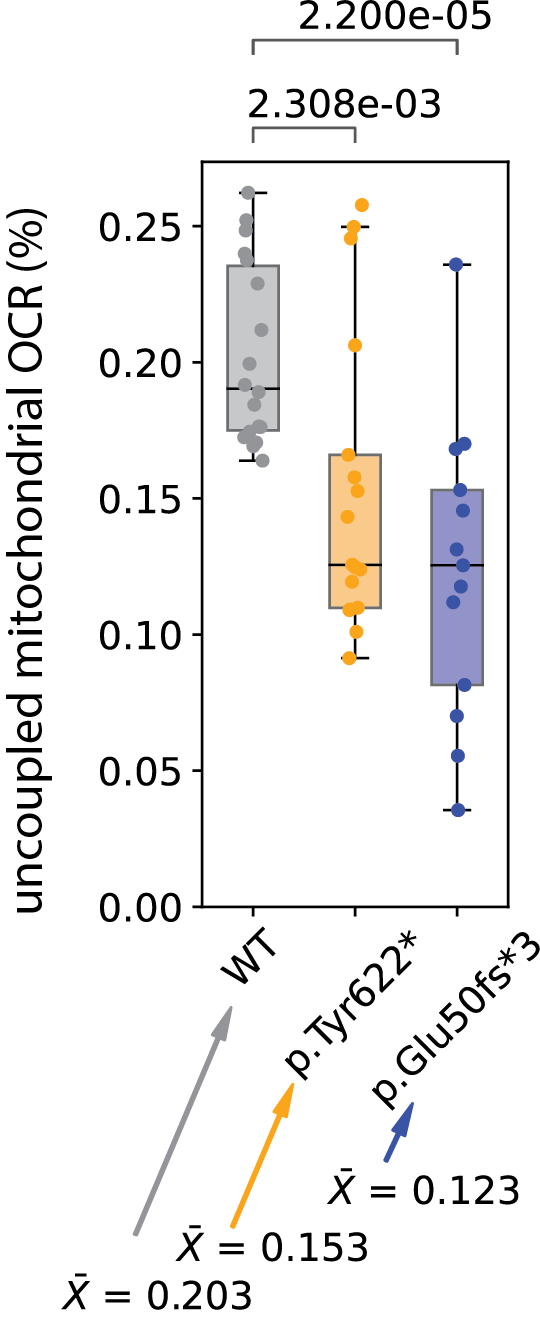
\includegraphics[width=\textwidth]{./main_plots/uncoupling.png}        
    \end{subfigure}   
    \begin{subfigure}[t]{.5\textwidth}
        \caption{}
        \includegraphics[width=\textwidth]{./extended_plots/mitohealth_y_g.png}        
    \end{subfigure}    
    % Row 3
    \begin{subfigure}[t]{.35\textwidth}
        \caption{}
        \includegraphics[width=\textwidth]{./main_plots/tmrm_main.png}        %tmrm_with_FCCP
    \end{subfigure}    
   % \hspace{1cm}
    \hspace{.25cm}
    \begin{subfigure}[t]{.35\textwidth}
        \caption{}
        \includegraphics[width=\textwidth]{./main_plots/cellrox_images.png}        
    \end{subfigure}  
    \hspace{.5cm}
    \begin{subfigure}[t]{.2\textwidth}
        \caption{}
        \includegraphics[width=\textwidth]{./main_plots/all_lipids_y622.png}        
    \end{subfigure}  
    \caption{
        \textbf{ABCA7 LoF Impacts Regulation of Mitochondrial Uncoupling in Neurons.}\\
    }
    \label{fig:main_mitochondrial}
\end{figure}
\begin{itemize}
    \item[\textbf{(A)}] Schematic of iPSC-derived isogenic neuronal lines harboring ABCA7 loss-of-function (LoF) variants. Gene structure shows exons (black rectangles) and introns (black lines). CRISPR-Cas9 introduced premature termination codons in exon 3 (p.Glu50fs3, blue) or exon 15 (p.Tyr622*, orange). Confocal images show MAP2 staining in iNs differentiated for 4 weeks (genotypes indicated).
    \item[\textbf{(B)}] Correlation of gene perturbation scores ($S = -\log_{10}(p)\times\text{sign}(\log_2(\text{FC}))$) by bulk mRNAseq comparing p.Glu50fs3 vs. WT and p.Tyr622* vs. WT iNs cultured for 4 weeks.
    \item[\textbf{(C)}] Kernighan-Lin (K/L) clustering of leading-edge genes from significantly perturbed pathways (Benjamini–Hochberg (BH) FDR-adjusted $p<0.05$) in p.Tyr622* vs. WT iNs. Colors represent distinct K/L clusters.
    \item[\textbf{(D)}] Heatmap of Jaccard index overlap between K/L gene clusters from p.Tyr622* neurons and clusters identified in human postmortem excitatory neurons. Red text denotes clusters with average score $S$ upregulated in ABCA7 LoF; blue text denotes clusters with average $S$ downregulated in ABCA7 LoF.
    \item[\textbf{(B)}] Heatmap showing Jaccard index overlap between K/L clusters identified in p.Glu50fs* vs. WT iNs and p.Tyr622* vs. WT iNs.
    \item[\textbf{(E)}] Gaussian kernel density plots of gene perturbation scores ($S$) within each cluster. Positive $S$ indicates upregulation in p.Tyr622*. Solid lines denote cluster means. Top enriched pathways with highest intra-cluster connectivity indicated.
    \item[\textbf{(F)}] Volcano plot of differential expression of genes with mitochondrial-localized protein products (MitoCarta) between p.Tyr622* and WT neurons.
    \item[\textbf{(G)}] Seahorse-measured mitochondrial uncoupled oxygen consumption rate (OCR) in WT and ABCA7 LoF and WT iNs cultured for 4 weeks. Each datapoint represents OCR from a single well. $N=18$ (WT), $17$ (p.Tyr622*), $13$ (p.Glu50fs3) wells, across two differentiation batches. Statistical comparison by independent-sample $t$-test.
    \item[\textbf{(H)}] Mitochondrial membrane potential quantified via HCS MitoHealth dye fluorescence intensity in ABCA7 LoF iNs cultured for 4 weeks. Each datapoint represents average intensity per well (NeuN+ volumes averaged). Statistical comparison via linear mixed-effects model, accounting for well-of-origin random effects. $N=8$ (WT), $11$ (p.Tyr622*), $9$ (p.Glu50fs3) wells; $\approx3000$ cells/condition, from three differentiation batches.
    \item[\textbf{(I)}] Baseline mitochondrial membrane potential quantified by average TMRM fluorescence intensity per masked region (thresholded at 75th percentile) in ABCA7 LoF and WT iNs cultured for 4 weeks. Each datapoint represents average intensity per well. $N=4$ (WT), $5$ (p.Tyr622*) wells. Statistical comparison by independent-sample $t$-test.
    \item[\textbf{(J)}] Oxidative stress quantified by average CellROX fluorescence intensity per masked region (thresholded at 75th percentile) in p.Tyr622* and WT iNs cultured for 4 weeks. Each datapoint represents average intensity per well. $N=10$ wells per genotype. Statistical comparison by independent-sample $t$-test.
    \item[\textbf{(K)}] Volcano plot of differentially abundant lipid species between p.Tyr622* and WT iNs cultured for 4 weeks, colored by lipid class. Statistical comparisons by independent-sample $t$-tests followed by BH FDR adjustment.
\end{itemize}
